\subsubsection{Construction du \ac{DODAG}}

\begin{figure}[ht]
  \centering
  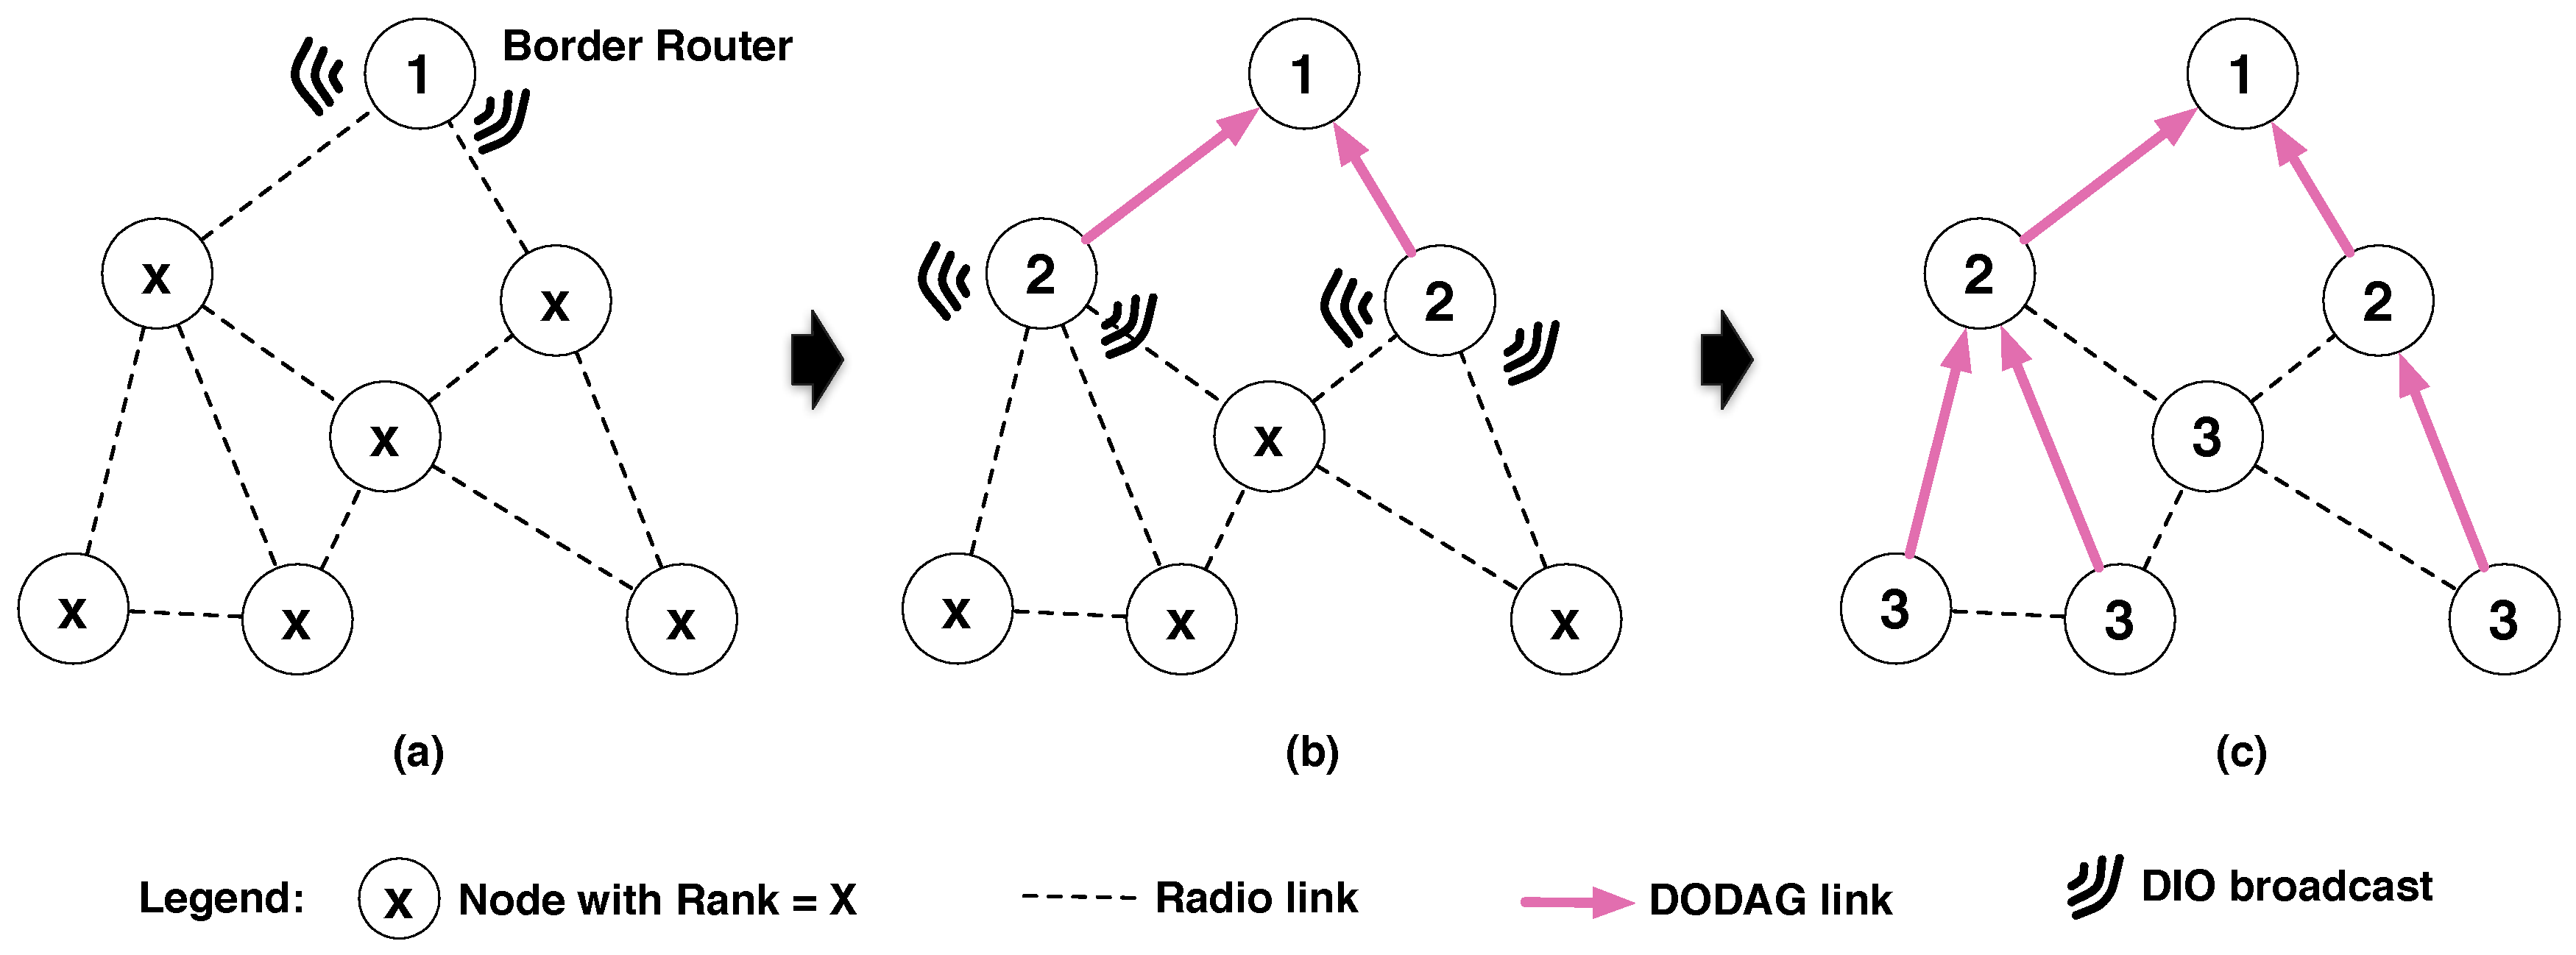
\includegraphics[width=\linewidth]{img/dodag.pdf}
  \caption{Construction d'un \ac{DODAG} (Figure à traduire)}
  \label{gw:fig:rpl_construction}
\end{figure}

Le \ac{LBR} est à la fois la racine de l'arbre de routage, la passerelle vers l'extérieur mais également le nœud collecteur de données.
Le processus de construction du \ac{DODAG} démarre au \ac{LBR} qui a un rang de 1 comme  représenté dans la figure~\ref{gw:fig:rpl_construction}.
La racine envoie un \ac{DIO} en multicast aux nœuds qui sont à portée de transmission.
Lorsqu'un nœud reçoit une nouvelle version de \ac{DIO}, il met à jour son rang par rapport au \ac{DIO} qu'il vient de recevoir en prenant un rang strictement plus grand en incrémentant d'une quantité fixe le rang qu'ils reçoivent.
Dans le cas de la figure~\ref{gw:fig:rpl_construction} l'incrément est de 1 les enfants de la racine ont donc un rang de 2.
La notion de rang est utilisée par \ac{RPL} notamment pour éviter les boucles~\cite{rfc6550}.

Si le nœud est configuré pour agir comme routeur il propage à son tour un \ac{DIO} en indiquant son rang.
Si le nœud n’est pas configuré pour être un routeur alors il rejoint tout simplement la structure \ac{DODAG} et n’envoie pas de \ac{DIO}.
Ce processus continue jusqu’à couvrir tous les nœuds du réseau.

Pour un nœud, tous les nœuds à portée de transmission qui ont un rang inférieur au sien peuvent devenir des parents.
Les parents optimaux sont obtenus à partir de fonctions objectives qui peuvent prendre plusieurs critères en compte comme la qualité du lien ou bien des paramètres d'\ac{ETX}~\cite{rfc6550}.
Chaque nœud de la structure \ac{DODAG} a une entrée de routage vers son parent (ou plusieurs parents selon la fonction d’objectif) à travers lequel ce nœud peut atteindre la racine de la structure \ac{DODAG}.

Les \ac{DAO}s sont quant à eux émis par des nœuds vers leurs parents pour annoncer les enfants qu'ils ont.
Ainsi il est possible de faire remonter jusqu'à la racine les routes descendantes et connaître la totalité de la topologie.
La remontée des routes est nécessaire dans les scénarios nécessitant l'envoi de trafic de type point à multi-point (La passerelle envoyant des paquets vers les nœuds) et point-à-point (Les nœuds communiquent entre eux).

\subsubsection{Réparation globale et locale}

\ac{RPL} dispose de deux mécanismes de réparation:

Le premier mécanisme est local, lorsqu'un nœud détecte une incohérence, il se détache du \ac{DODAG} en se mettant à un rang infini ce qui ``empoisonne'' ses routes.
Les enfants le détecte et le retire de leur liste de parents avant une reconstruction des routes.

Le second mécanisme est global.
Il reconstruit l'intégralité du \ac{DODAG}.
La racine incrémente la version du \ac{DODAG} id qu'elle propose, les nœuds propagent ce changement et reconstruisent un nouveau \ac{DODAG}.

\subsection{Limitation de la signalisation de routage}

\subsubsection{Trickle}

\ac{RPL} utilise un mécanisme de timer adaptatif appelé  ``Trickle'' (goutte à goutte) afin de contrôler le débit d’émission des \ac{DIO}s.
Trickle double l’intervalle séparant deux émissions successives de paquets \ac{DIO} à chaque fois que le réseau est cohérent, et ce jusqu’à une valeur maximale.
Ainsi le trafic \ac{RPL} diminue dans le réseau lorsqu'il est stable.
Quand une incohérence est détectée, le timer est réinitialisé à sa valeur minimale.
Un des principaux avantages de l’utilisation du timer Trickle est qu’il ne nécessite pas de code complexe et il est assez facile à mettre en œuvre.
La convergence de Trickle vers le temps inter \ac{DIO} maximal peut être difficile dans des conditions réelles de transmissions~\cite{tripathi2010performance}.


\subsubsection{Détection et évitement des boucles}

\ac{RPL} est proactif et ne garantit pas un routage sans boucle ou de garantie sur les délais de convergence.
Ce choix est acceptable dans des scénarios de smart metering dans lequel un délai supplémentaire occasionnel des paquets n'est pas critique~\cite{yan2013survey} mais peut être dommageable dans des scénarios ou des délais plus stricts sont requis.
Cependant \ac{RPL} dispose de plusieurs mécanismes pour éviter les boucles de routage par des mécanismes de détection, de réparation globale et locale et en diminuant son rythme de surveillance à mesure que le réseau se stabilise.


Les règles utilisées par \ac{RPL} pour éviter les boucles utilisent le rang précédemment introduit.
Lors de la désignation d'un parent, un nœud ne peut sélectionner qu'un voisin qui a un rang plus faible que le sien.
De plus, il n'est pas possible de réduire son rang pour augmenter artificiellement le nombre de parents potentiels.

Dans le cas où \ac{RPL} fonctionne avec stockage, il est possible d'utiliser les entêtes pour spécifier si le trafic est montant ou descendant.

Dans le cas où \ac{RPL} fonctionne sans stockage, la racine détecte au moment de l'envoi si un routeur apparaît plus d'une fois dans le chemin emprunté.

\paragraph{Tables de routage}

Afin de gérer les tables de routage, \ac{RPL} peut fonctionner selon deux manières: avec et sans stockage des routes.

Lorsque les routes sont stockées, une table de routage doit être construite au niveau de chaque nœud vers.

Dans le cas où les routes ne sont pas stockées, seul la racine reçoit et traite messages de routage des nœuds et ainsi seul la racine connaît le chemin vers chaque destination.
Ainsi pour atteindre un nœud, le routage est précisé explicitement par la racine.
% Dans le cas du \ac{P2P}, tout le trafic remonte à la racine.
Ce cas d'utilisation est recommandé dans le cas de nœuds suffisamment contraint pour ne pas pouvoir gérer une table de routage.

% % Cette tâche est accomplie par les \ac{DAO}s qui sont utilisés pour annoncer les nœuds qui peuvent être des destinations potentielles dans du trafic descendant.
% % Un nœud appartenant à la structure \ac{DODAG} enverra un \ac{DAO} à ses parents.
% % À la réception de ce  \ac{DAO}, un nœud parent ajoute une entrée dans la table de routage et il envoie à son tour un \ac{DAO} à ses parents\footnote{des agrégations des informations reçues peuvent être envisagées} jusqu’à ce que l’information atteigne la racine du \ac{DODAG}.
% % Dans ce cas, lorsque du trafic \ac{P2P} doit être routé, les paquets remontent jusqu'à un nœud en commun puis sont routés depuis cet ancêtre commun.

% \paragraph{Routage de bordure}

% Dans les cas d'applications usuels des \ac{LLN}, le trafic sort des nœuds vers un réseau local ou bien vient du réseau local et va vers les nœuds.
% Ainsi le routage de bordure se produisant à la passerelle est particulièrement important car l'essentiel du trafic passera par ce routeur qui est également appelé passerelle.

% Dans les cas les plus simples, il y a qu'un seul routeur de bordure pour le \ac{LLN} et le préfixe du \ac{LLN} est différent de celui de son interface IPv6.
% Ainsi le routeur de bordure ne route pas les paquets non pertinents pour le \ac{LLN} vers lui.
% Il est à noter que le routeur de bordure peut exécuter un protocole de routage pour le \ac{LLN} et un autre pour son autre réseau par exemple \ac{OSPF}.
% Dans ce cas, il est nécessaire de procéder à une redistribution de routes où le routeur de bordure annonce des routes maintenue à l'autre.
% Puisque les \ac{LLN} sont essentiellement des ``stub-network'' l'annonce des routes va essentiellement du \ac{LLN} vers le réseau classique car les \ac{LLN} n'ont pas vocation a router un trafic qui n'est pas le leur.


% \paragraph{Routage interne au \ac{LLN}}

% \ac{RPL} maintient une topologie permettant de gérer le trafic ascendant (\ac{MP2P}) c'est à dire celui permettant aux nœuds du \ac{LLN} de router leurs paquets vers le routeur de bordure.
% Le second mécanisme de routage descendant (\ac{P2MP}) permet de faire remonter toutes les routes de la topologie vers le routeur de bordure afin de permettre le trafic descendant allant du routeur de bordure vers les nœuds.

% La fiabilité de ce routage est améliorée par l'utilisation potentielles de plusieurs routeurs permettant de choisir dynamiquement la route choisie.
% Quand un nœud souhaite envoyer un paquet vers une destination non accessible depuis son lien local, il l'envoie à son parent préféré, puis cette transmission échoue a ses autres parents.
% Les parents potentiels sont classés au moment de la construction des routes et selon la métrique choisie, le meilleur parent est choisi.

% Le routage descendant peut être obtenu par l'utilisation d'un vecteur de distance à chaque saut dans le cas par défaut ou par  routage à la source dans le cas où c'est le routeur de bordure qui le spécifie par exemple pour des raisons d'espace de stockage disponible sur chaque routeur intermédiaire.

% Puisque l'essentiel du trafic est \ac{MP2P} ou bien \ac{P2MP}, la structure de routage optimal est un graphe qui pointe vers les points de sortie du réseau que sont les routeurs de bordure.
% Pour se construire les nœuds ont besoin d'envoyer des informations spécifiques (profondeur, coût, \ldots).
% En utilisant des métriques et des fonctions objectives définies, les nœuds sont capables de choisir parmi un ensemble de voisins, leur parent qui va envoyer le trafic vers le routeur de bordure.
% Cette topologie contruit automatiquement les chemins des nœuds vers les routeurs de bordure qui peut être utilisé pour le trafic montant.
% De plus, elle est maintenue par l'envoi de signalisation périodique envoyé par le routeur de bordure vers les nœuds puis propagée par chaque routeur du \ac{LLN}.
